\documentclass{article}
\usepackage[utf8]{inputenc}
\usepackage{float}
\usepackage{natbib}
\usepackage{graphicx}
\usepackage{hyperref}
\usepackage{minted}
\hypersetup{
    colorlinks=true,
    linkcolor=blue,
    filecolor=magenta,      
    urlcolor=cyan,
}

\newcommand{\concatenatedInputs}{\textit{concatenatedInputs }}

\title{ARM Exercise 1 Report}

\author{Tsotne Putkaradze}
\date{7 October 2015}
\linespread{0.3}
\begin{document}
\maketitle


\section{Task Given}
Write a piece of Synthesizable Verilog design to generate the following outputs when a "Go" pulse is observed at the inputs. OutD is generated synchronous to clk\_in. The "Z" in the waveform suggests that the output is in high impedance state.

\begin{figure}[H]
\centering
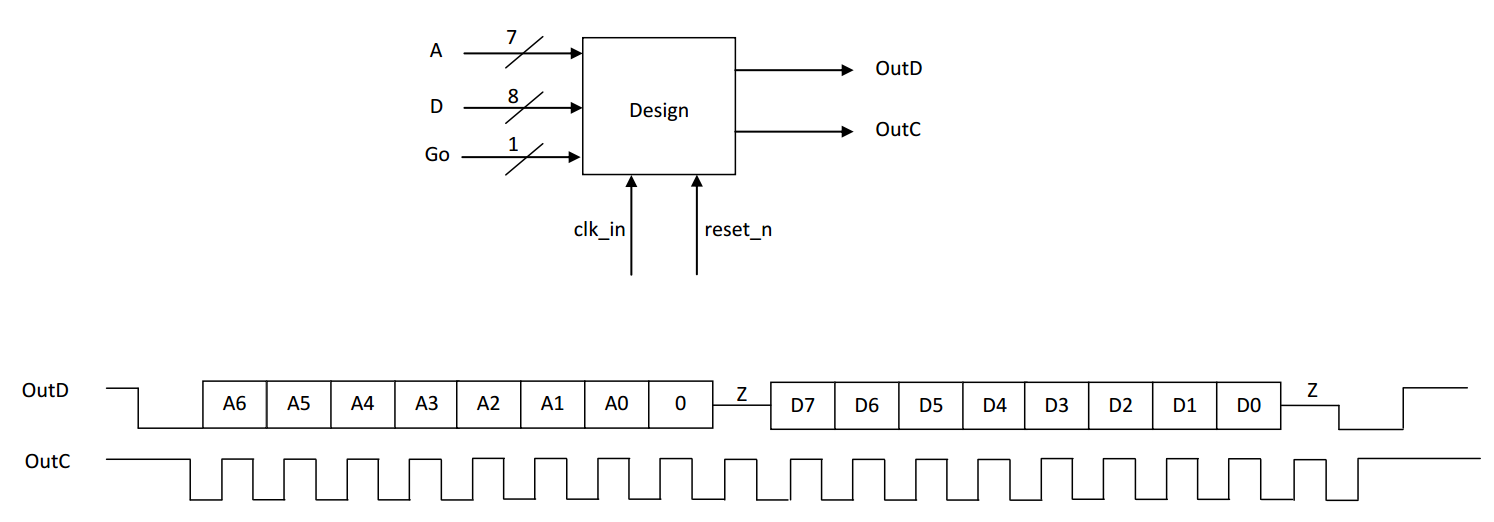
\includegraphics[width=\textwidth] {task_arm.png}
\caption{task given}
\label{fig:task_arm}
\end{figure}

According to fig: \ref{fig:task_arm} (if circuit is designed on rising edge)
\begin{enumerate}
\item First value receiver "clocks" is Highest(Left Most) Bit of A input
\item Last Value receiver "clocks" is '0' 
\end{enumerate}

\newpage
\section{Solution}
Until writing code, I came up with two possible solutions that are: 
\begin{itemize}
\item Solution A : using 19bit-shift register
\item Solution B : using 3bit-counter with FSM
\end{itemize}

Verilog solutions were simulated using Open Source Software: Icarus Verilog.
Both, Verilog and VHDL solutions were synthesized and simulated using Vivado 2015 Synthesis and Simulation Tools, with Tallinn University of Technology Licence. 


\subsection{Solution A : Solution With Shift Register}
Circuit works like this: after Go signal arrives, shift register "\concatenatedInputs" receives value: 
\newline $ '0' + A(7bitInput) + 'Z' + D(8bitInput) + 'Z' + '0' $ \newline
and on every clock cycle we do following: \newline
\begin{itemize}
\item on output OutD, we send out \concatenatedInputs[Left\_Most\_Bit]
\item vector \concatenatedInputs is shifted to the left and '1' is inserted from right side ('1' is because in idle state our output should be '1' anyways, so when \concatenatedInputs will be shifted "1+7+1+8+1+1"-times output will be constant '1', because shift register will consist of only '1's. output will be '1' until we reset the circuit or give it new input (with Go signal).
\item we observe value of \concatenatedInputs, if it consists of all 1s, then we stop propagating clk\_in into OutC.
\end{itemize}
With this solution I don't have to use any adder, fsm or any other relatively complicated logic. 


\subsection{Solution B : Solution With 3bit Counter and FSM}
This solution is following, after Go signal arrives, we store the data in registers. We construct one - 3 bit adder. we use this adder to address the correct bit of stored inputs, like this: \newline
$ OutD <= stored_Input_A [counterValue]; $
and FSM controls which vector will be sent to output, $stored_Input_A$ or $stored_Input_D$


\section{Decision}
However I decided to write code for solution A, because it looked much simpler in circuit point of view, i was using registers, that was definitely necessary to use(unless inputs are not changing during transmission of data), and i am using them as shift register, so I'm not adding anything heavy.

First I wrote VHDL code because i have VHDL background, then i learnt Verilog and wrote the code there.

In both solutions everything is parametrised: length of delay before and after inputs, length of high impedance output, length of input A and input D.

P.S.
In attached files, there is also folder called "Additional" there, I've constructed circular serial communication between N number of FPGAs, there I've used the logic of Solution B - storing vector and selecting right bit with counter value.

\section{Verification}
For validating the correctness of logic, in both languges I generated test-benches, that take both output OutD and OutC, and reconstruct the provided data, in other words, we use OutC as a clock to sample/receive OutD. and I used Assert statements to compare the provided and reconstructed data.

\section{Simulation}
On the figures below, you can see the simulations when following inputs are given:
$A = 1000001, D = 10000001$
Codes are also synthesizable, you can view the synthesis reports in corresponding folders

\begin{figure}[H]
\centering
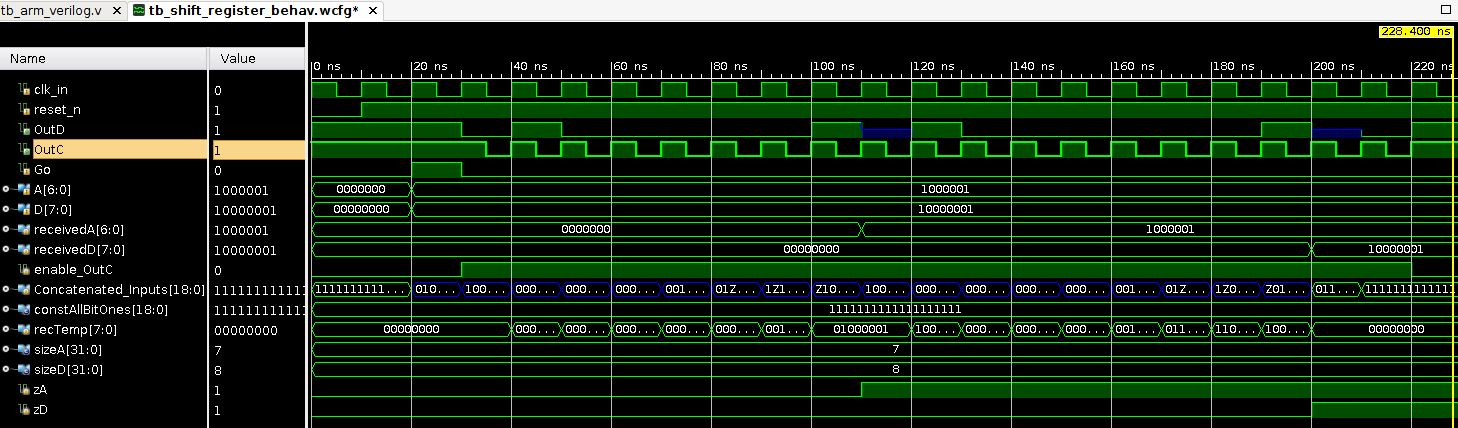
\includegraphics[width=\textwidth] {tb_verilog.png}
\caption{waveform of outputs generated from above mentioned inputs, logic is written in Verilog Language, simulation tool: Vivado 2015.2}
\label{fig:tb_verilog}
\end{figure}

\begin{figure}[H]
\centering
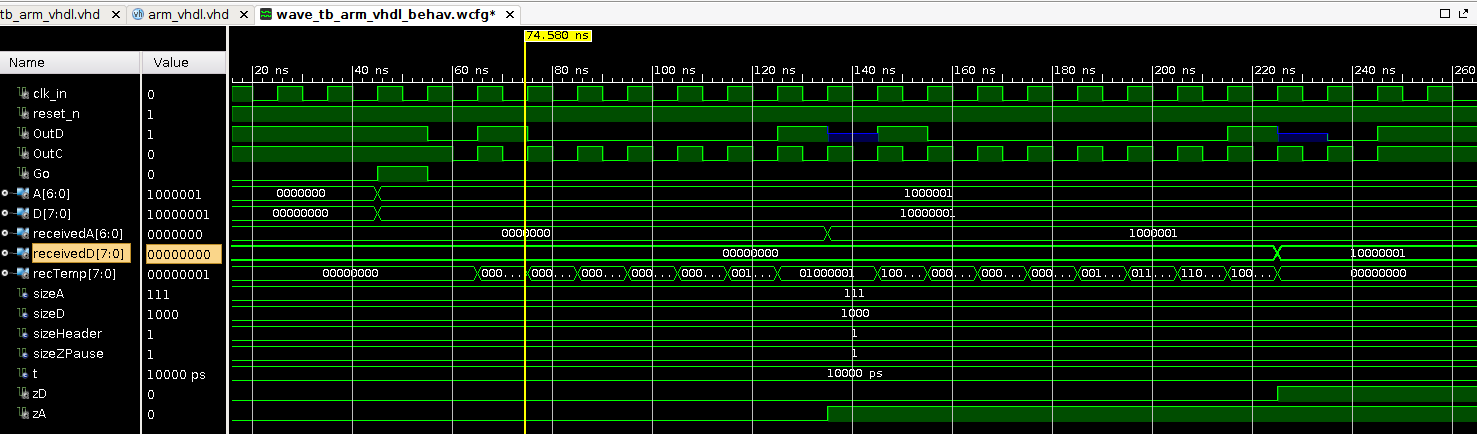
\includegraphics[width=\textwidth] {tb_vhdl.png}
\caption{waveform of outputs generated from above mentioned inputs, logic is written in VHDL Language, simulation tool: Vivado 2015.2}
\label{fig:tb_vhdl}
\end{figure}

\begin{figure}[H]
\centering
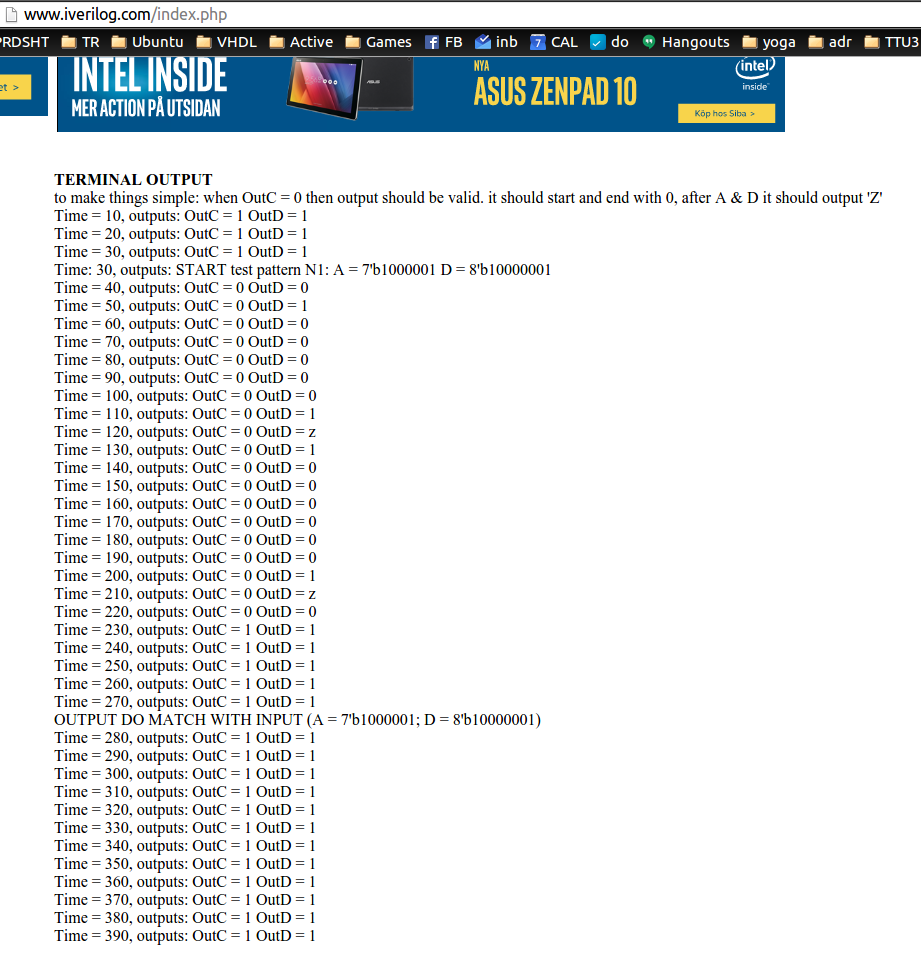
\includegraphics[width=\textwidth] {tb_iverilogcom.png}
\caption{waveform of outputs generated from above mentioned inputs, logic is written in Verilog Language, simulation tool: Icarus Verilog - www.iverilog.com}
\label{fig:tb_iverilogcom}
\end{figure}

\begin{figure}[H]
\centering
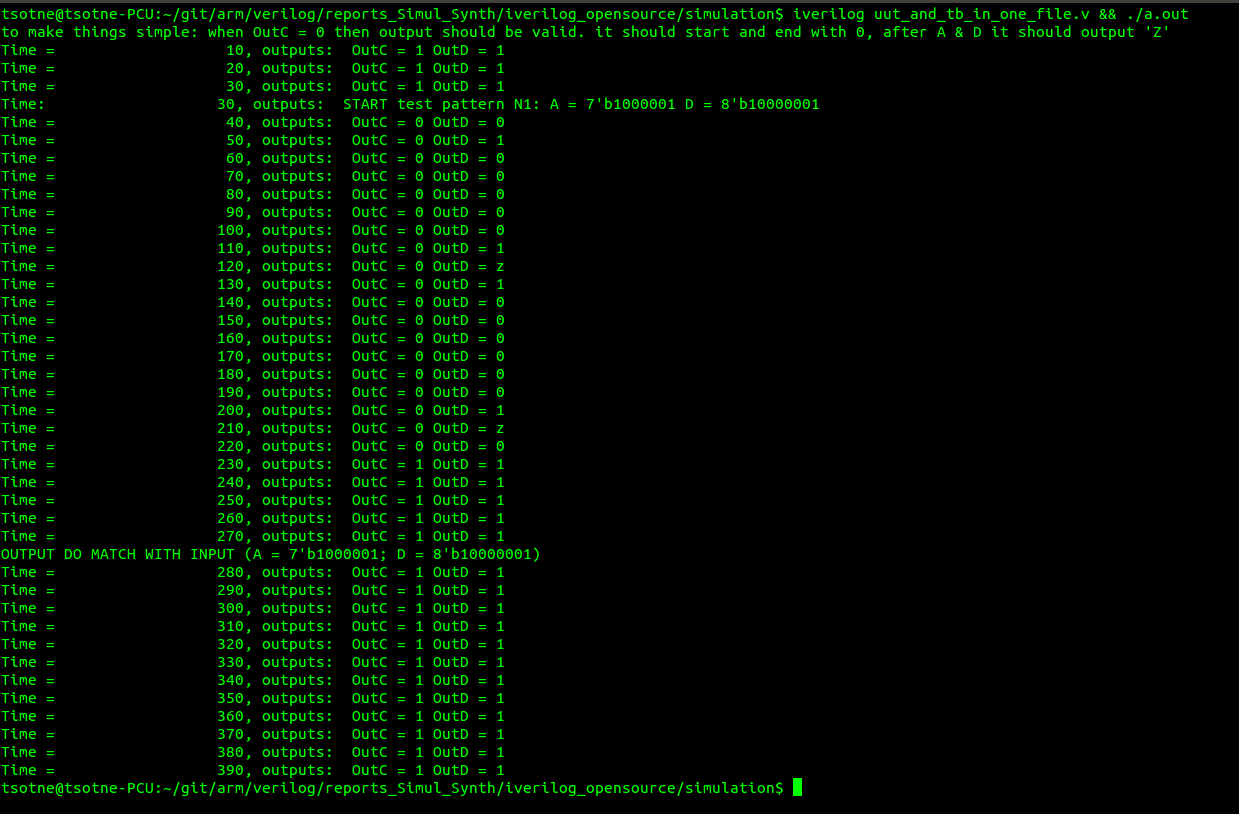
\includegraphics[width=\textwidth] {tb_iveriloglinux.png}
\caption{waveform of outputs generated from above mentioned inputs, logic is written in Verilog Language, simulation tool: Icarus Verilog - www.iverilog.icarus.com}
\label{fig:tb_iverloglinux}
\end{figure}


\bibliographystyle{plain}
\bibliography{references}
\end{document}